\begin{figure}
	\begin{center}
	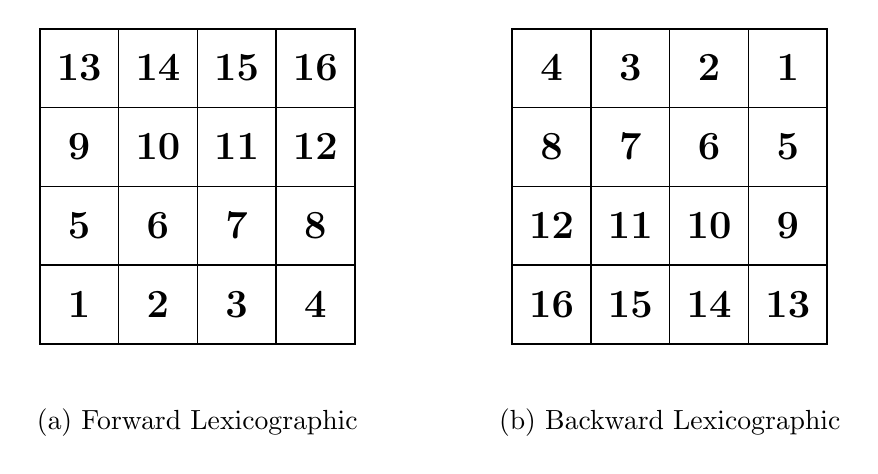
\begin{tikzpicture}[scale=4] 
	

\def\n{4} % Number of divisions
\def\step{0.25} % Step size (1/n since domain is [0,1]x[0,1])

    % Draw the grid
\draw[thick] (0,0) rectangle (1,1); % Outer square
\foreach \i in {1,2,3} {
        \draw[thin] (\i*\step,0) -- (\i*\step,1); % Vertical lines
        \draw[thin] (0,\i*\step) -- (1,\i*\step); % Horizontal lines
    }

    % Number the cells
    \foreach \row in {0,1,2,3} {
        \foreach \col in {0,1,2,3} {
            \node at ({(\col+0.5)*\step},{(\row+0.5)*\step}) {\Large \bfseries \the\numexpr 1 + \col + 4*\row};
        }
    }
    
    \def\n{4} % Number of divisions
    \def\step{0.25} % Step size (1/n since domain is [0,1]x[0,1])

    % Draw the grid
    \draw[thick] (1.5,0) rectangle (2.5,1); % Outer square
    \foreach \i in {1,2,3} {
        \draw[thin] (\i*\step+1.5,0) -- (\i*\step+1.5,1); % Vertical lines
        \draw[thin] (1.5,\i*\step) -- (2.5,\i*\step); % Horizontal lines
    }

    % Number the cells
    \foreach \row in {0,1,2,3} {
        \foreach \col in {0,1,2,3} {
            \node at ({(\col+0.5)*\step+1.5},{(\row+0.5)*\step}) {\Large \bfseries \the\numexpr 1 + (3-\col) + 4*(3-\row)};
        }
    }
\node at (0.5, -0.25) {(a) Forward Lexicographic};
\node at (2.0, -0.25) {(b) Backward Lexicographic};
    
	\end{tikzpicture}
	\end{center}
	\caption[Lexicographic enumerations.]{(a) Forward lexicographic and (b) backward lexicographic enumeration of the cells of a $4\times 4$ grid.}
	\label{fig-lexicographic}
	\end{figure}
